%% ID: three_collisions
%% TITLE: Three Collisions
%% TYPE: question
%% QUESTIONTYPE: symbolic
%% CONCEPTS: energy, momentum
%% VIDEOS: 
%% LEVEL: 3
%% TOPIC: mechanics/dynamics
%% ORDER: 8

\begin{problem}[A1969AMIIQ8l] %Standard multiple collision. Coefficient of restitution exorcised.
{Three particles A, B, and C, each of mass \vari{m}, lie at rest in that order in a straight line on a smooth horizontal table. The particle A is then projected directly towards B with speed \vari{u}. 
\begin{enumerate}
	\item Find the velocities of the three particles immediately after the second impact, assuming the collisions are perfectly elastic.
\end{enumerate}
The masses of A, B, and C are now \vari{m}, \vari{2m} and \vari{3m} respectively:
\begin{enumerate}[resume]
	\item Again find the velocities of the three particles immediately after the second impact, assuming the collisions are perfectly elastic.
	\item What is the velocity of the composite particle after the second impact, if the balls now collide completely inelastically?
\end{enumerate}

\emph{Hint:} Draw several diagrams.
\begin{enumerate}
	\item In a completely elastic collision, no kinetic energy is lost.
	\item Completely inelastically means that the particles stick together to form a new particle of mass \value{m_{new}}{{m_{1} + m_2}}{}.
\end{enumerate}
}
{\textit{Used with permission from UCLES, A Level Applied Mathematics, June~1969, Paper~2, Question~8.}}
{To solve each part of this question we consider each collision in turn, staying in general symbols for each collision for as long as possible. Draw a diagram of the system before each collision, noting that as in Figure \ref{fig:Dynamics_ball_collisions} the third ball in each case need not be drawn since it is not involved. Writing the initial velocity above the diagram, and the final velocity below the diagram, is a useful way of keeping track of collisions and has been done in the Figure. 

We will use the magnitude of velocity (i.e. the speed) throughout the solution, rather than vectors; but in the second part of the solution when the particles no longer all move in the same direction, a negative speed denotes the opposite direction to the initial speed \vari{u}. This is an oft used convention for 1D problems, where the minus sign acts to give the direction and the number gives the magnitude of what should be a vector quantity.

\begin{figure}[h]
  \centering
%	\begin{subfigure}{0.5\textwidth}
%	\centering
 	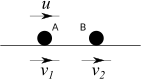
\includegraphics[width=0.5\linewidth]{../../../figures/Dynamics_ball_collision_AB.eps}
	\caption{}
	\label{fig:Dynamics_ball_collision_AB}
%	\end{subfigure}%
	%\begin{subfigure}{0.5\textwidth}
\end{figure}
\begin{figure}[h]
	\centering
	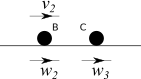
\includegraphics[width=0.5\linewidth]{../../../figures/Dynamics_ball_collision_BC.eps}
	\caption{}
	\label{fig:Dynamics_ball_collision_BC}
	%\end{subfigure}
\caption{}
%\label{fig:Dynamics_ball_collisions}
\end{figure}

\begin{enumerate}
	\item Conserving momentum and conserving energy will give two simultaneous equations which can then be solved for the two unknowns \vari{\vtr{v}_{1}} and \vari{\vtr{v}_{2}}.
Conserve momentum:
\begin{align} \notag 
(m)(u) + (m)(0) &= (m)(v_{1}) + (m)(v_{2}) \\ u &= v_{1} + v_{2} \label{Ball_AB_CoM}
\end{align}
Conserve energy:
\begin{align} \notag 
\frac{1}{2}mu^{2} &= \frac{1}{2}mv_{1}^{2} + \frac{1}{2}mv_{2}^{2} \\ u^{2} &= v_{1}^{2} + v_{2}^{2} \label{Ball_AB_CoE}
\end{align}
Then solving \ref{Ball_AB_CoM} and \ref{Ball_AB_CoE} as simultaneous equations gives two solutions. Looking at the two solutions, it is clear that the solution where \value{v_{1}}{u} and \value{v_{2}}{0}{m\,s\sup{-1}} is the initial condition before the collision. Thus the other solution gives the situation after the collision: \value{v_{1}}{0}{m\,s\sup{-1}} and \value{v_{2}}{u}.

Repeating this process exactly but for the second collision, Figure \ref{fig:Dynamics_ball_collision_BC}, and leaving \vari{v_{2}} unsubstituted, gives simultaneous equations:
\begin{align} 
v_{2} &= w_{2} + w_{3} \label{Ball_BC_CoM} \\  
v_{2}^{2} &= w_{2}^{2} + w_{3}^{2} \label{Ball_BC_CoE}
\end{align}
where again \ref{Ball_BC_CoM} comes from conserving momentum and \ref{Ball_BC_CoE} comes from conserving energy. Solving these gives \value{w_{2}}{0}{m\,s\sup{-1}} and \vari{w_{3}} = \value{v_{2}}{ u}{}, with the same reasoning as before applying.

We now have the three velocities:
\begin{align*}
 v_{1} = 0 && w_{2} = 0 && w_{3} = u 
\end{align*}
as the final velocities of the three balls.


	\item This part is very similar to the first part, but now the masses must be included in the simultaneous equations for each collision. Considering the first collision, conserve momentum:
\begin{align} \notag 
(m)(u) + (2m)(0) &= (m)(v_{1}) + (2m)(v_{2}) \\ 
u &= v_{1} + 2v_{2} \label{Ball_AB_CoM_uneq} 
\end{align}
and energy:
\begin{align} \notag 
\frac{1}{2}mu^{2} &= \frac{1}{2}mv_{1}^{2} + \frac{1}{2}(2m)v_{2}^{2} \\ 
u^{2} &= v_{1}^{2} + 2v_{2}^{2} \label{Ball_AB_CoE_uneq} 
\end{align}
Solving \ref{Ball_AB_CoM_uneq} and \ref{Ball_AB_CoE_uneq} again produce two solutions; the initial condition and the result after the collision. The simultaneous equations involved the speeds, but the solution for \vari{v_{1}} is negative. A negative speed is non-physical, but indicates that the direction of motion has reversed. The speeds after the collision are \value{v_{1}}{- \frac{1}{3}u}{} and \value{v_{2}}{\frac{2}{3}u}{}.

As before, repeating the process for the second collision gives two equations:
\begin{align*} 
2v_{2} &= 2w_{2} + 3w_{3} \\
 2v_{2}^{2} &= 2w_{2}^{2} + 3w_{3}^{2} 
 \end{align*}
with solution for after the collision of \vari{w_{2}} = \value{- \frac{1}{5} v_{2}}{- \frac{2}{15} u}{} and \vari{w_{3}} = \value{\frac{4}{5} v_{2}}{\frac{8}{15} u}{}. Thus the final speeds after the second collision are:
\begin{align*} 
v_{1} = - \frac{1}{3}u && w_{2} = - \frac{2}{15}u && w_{3} = \frac{8}{15}u 
\end{align*}
	\item Finally the completely inelastic collision, where the balls coalesce on impact. This leaves only one unknown and so we only need to consider momentum, which is good because kinetic energy is not conserved in inelastic collisions.
Considering the first collision and conserve momentum:
\begin{align*} 
(m)(u) + (2m)(0) &= (m + 2m)(v_{1}) \\
 u &= 3v_{1} \\ 
 v_{1} &= \frac{1}{3}u 
 \end{align*} 
 and both particles move together at that speed.
Consider the second collision and again conserve momentum:
\begin{align*} 
(m + 2m)(v_{1}) + (3m)(0) &= (m + 2m + 3m)(v_{f}) \\ 
3v_{1} &= 6v_{2} \\ 
v_{f} &= \frac{1}{2} v_{1} \\ 
v_{f} &= \frac{1}{6} u 
\end{align*}
This can also be simplified into one step, straight to the final speed of the composite particle \vari{v_{f}}, since momentum is conserved no matter how many intermediate collisions occur:
\begin{align*} 
(m)(u) + (2m)(0) + (3m)(0) &= (m + 2m + 3m)(v_{f}) \\ 
u &= 6 v_{f} \\ 
v_{f} &= \frac{1}{6} u 
\end{align*}
\end{enumerate}

}
\end{problem}